\documentclass[letterpaper, 12pt]{math}
\usepackage{pgfplots}

\pgfplotsset{compat=1.10}
\usepgfplotslibrary{fillbetween}
\usetikzlibrary{patterns}

\title{Areas Between Curves}
\author{Alvin Lin}
\date{Calculus II: August 2016 - December 2016}

\begin{document}

\maketitle

\section*{Areas Between Curves}

\begin{center}
  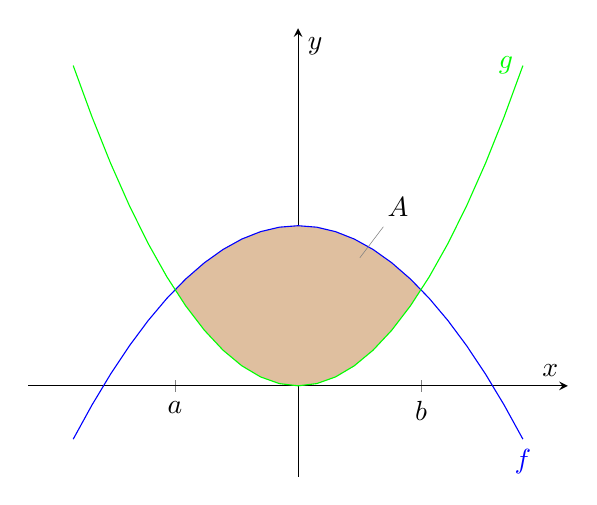
\begin{tikzpicture}
    \begin{axis}[axis lines=middle,
                 xlabel=\(x\),
                 ylabel=\(y\),
                 enlargelimits,
                 ytick=\empty,
                 xtick={-2.19,2.19},
                 xticklabels={\(a\),\(b\)}]
    \addplot[name path=F,
             blue,
             domain={-4:4}]{-(1/6)*x^2+2} node[pos=1, below]
             {\(f\)};
    \addplot[name path=G,
             green,
             domain={-4:4}]{0.25*x^2} node[pos=1, left]
             {\(g\)};
    \addplot[color=brown!50] fill between [
             of=F and G, soft clip={domain=-2.19:2.19}];
    \node[coordinate,pin=60:{$A$}] at (axis cs:1.1,1.6){};
    \end{axis}
  \end{tikzpicture}
\end{center}
Finding the area between curves is very similar to finding the area underneath
a curve. The area between \(f\) and \(g\) is simply the difference between the
area under \(f\) and the area under \(g\).
\[ A = \int_{a}^{b}{\bigg[f(x)-g(x)\bigg]\diff{x}} \]

\subsection*{Practice Problem 1}
Find the area between the curves:
\[ y = 5x-x^{2} \]
\[ y = x \]
\begin{center}
  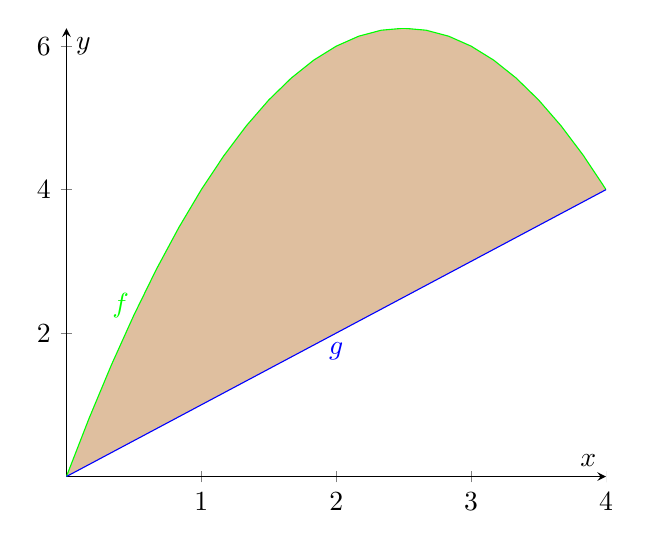
\begin{tikzpicture}
    \begin{axis}[axis lines=middle,
                 xlabel=\(x\),
                 ylabel=\(y\)]
    \addplot[name path=F,
             green,
             domain={0:4}]{5*x-x^2} node[pos=0.25, left]
             {\(f\)};
    \addplot[name path=G,
             blue,
             domain={0:4}]{x} node[pos=0.5, below]
             {\(g\)};
    \addplot[color=brown!50] fill between [
             of=F and G];
    \end{axis}
  \end{tikzpicture}
\end{center}
We need to find the points of intersection between the curves:
\[ x = 5x-x^{2} \]
\[ x^{2}-4 = 0 \]
\[ x(x-4) = 0 \]
\[ x = 0 \quad x = 4 \]
Now we can use those as the limits of integration:
\[ A = \int_{a}^{b}{\bigg[f(x)-g(x)\bigg]\diff{x}} \]
\[ A = \int_{0}^{4}{\bigg[5x-x^{2}-x\bigg]\diff{x}} \]
\[ \int_{0}^{4}{\bigg[4x-x^{2}\bigg]\diff{x}} \]
\[ \bigg[\frac{4x^{2}}{2}-\frac{x^{3}}{3}\bigg]_{0}^{4} \]
\[ \frac{4(4^{2})}{2}-\frac{4^{3}}{3}-(0-0) \]
\[ = 32 - \frac{64}{3} = \frac{32}{3} \]

\subsection*{Practice Problem 2}
Find the area between the curves:
\[ y = x \]
\[ y = x^{2} \]
\begin{center}
  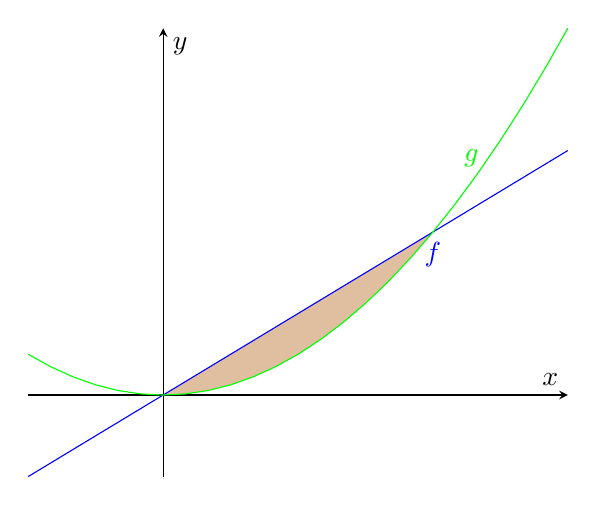
\begin{tikzpicture}
    \begin{axis}[axis lines=middle,
                 xlabel=\(x\),
                 ylabel=\(y\),
                 ytick=\empty,
                 xtick={0,4},
                 xticklabels={\(a\),\(b\)}]
    \addplot[name path=F,
             blue,
             domain={-0.5:1.5}]{x} node[pos=0.75, below]
             {\(f\)};
    \addplot[name path=G,
             green,
             domain={-0.5:1.5}]{x^2} node[pos=0.75, left]
             {\(g\)};
    \addplot[color=brown!50] fill between [
             of=F and G, soft clip={domain=0:1}];
    \end{axis}
  \end{tikzpicture}
\end{center}
We need to find the points of intersection between the curves:
\[ x = x^{2} \]
\[ x^{2}-x = 0 \]
\[ x(x-1) = 0 \]
\[ x = 0 \quad x = 1 \]
Now we can use these as the limits of integration:
\[ A = \int_{0}^{1}{x-x^{2}\diff{x}} \]
\[ \bigg[\frac{x^{2}}{2}-\frac{x^{3}}{3}\bigg]_{0}^{1} \]
\[ \frac{1}{2}-\frac{1}{3}-(0-0) \]
\[ = \frac{1}{6} \]

\subsection*{Practice Problem 7}
Find the area between the curves in the first quadrant:
\[ y = \sqrt{x} \]
\[ y = x-2 \]
This problem is trickier, we must split it into two integrals.
\begin{center}
  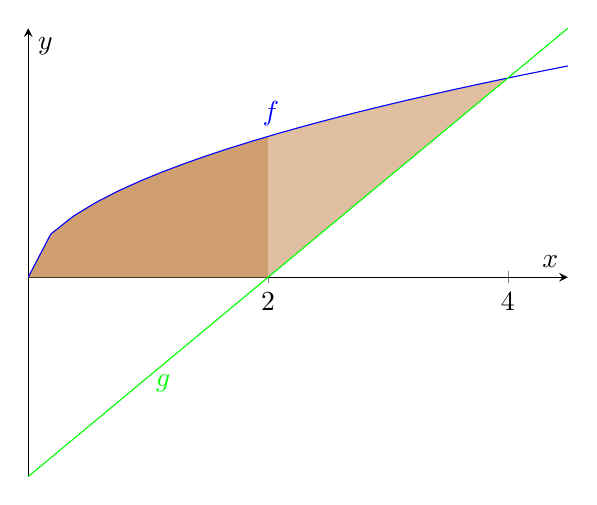
\begin{tikzpicture}
    \begin{axis}[axis lines=middle,
                 xlabel=\(x\),
                 ylabel=\(y\),
                 ytick=\empty,
                 xtick={2,4}]
    \addplot[name path=F,
             blue,
             domain={0:4.5}]{sqrt(x)} node[pos=0.5, above]
             {\(f\)};
    \addplot[name path=G,
             green,
             domain={0:4.5}]{x-2} node[pos=0.25, below]
             {\(g\)};
    \path[name path=axis] (axis cs:0,0) -- (axis cs:2,0);
    \addplot[color=brown!75] fill between [
             of=axis and F, soft clip={domain=0:2}];
    \addplot[color=brown!50] fill between [
             of=F and G, soft clip={domain=2:4}];
    \end{axis}
  \end{tikzpicture}
\end{center}
\[ A = \int_{0}^{2}{\sqrt{x}\diff{x}}+\int_{2}^{4}{\sqrt{x}-(x-2)\diff{x}} \]
The first integral is just the area under the curve of \( \sqrt{x} \) from 0 to
2, while the second integral is the area between the curves from 2 to 4.
\[ \bigg[\frac{2}{3}x^{\frac{3}{2}}\bigg]_{0}^{2}+
   \bigg[\frac{2}{3}x^{\frac{3}{2}}-\frac{1}{2}x^{2}+2x\bigg]_{2}^{4} \]
\[ \frac{2}{3}(2^{\frac{3}{2}})+
   \bigg[\frac{2}{3}4^{\frac{3}{2}}-\frac{1}{2}4^{2}+2(4)\bigg]-
   \bigg[\frac{2}{3}2^{\frac{3}{2}}-\frac{1}{2}2^{2}+2(2)\bigg] \]
\[ \frac{2}{3}(2^{\frac{3}{2}})+
   \frac{2}{3}4^{\frac{3}{2}}-\frac{1}{2}4^{2}+2(4)-
   \frac{2}{3}2^{\frac{3}{2}}+\frac{1}{2}2^{2}-2(2) \]
\[ \frac{16}{3}-8+8+4-4 \]
\[  = \frac{16}{3} \]

\begin{center}
  If any errors are found, please contact me at alvin.lin.dev@gmail.com
\end{center}

\end{document}
